%
% Serie von Laborexperiment haben wir den Nutzer verschiedene Aufgaben gestellt. Die Aufgaben werden immer komplexer
% und diese dann beobachtet                         - OK
% wie haben wir die Nutzer vorbereitet, geschult    - OK
% Wie haben arbeitsmaterialein ausgsehen            - OK
% Wie haben wir sie befragt                         - OK
% Was für daten haben wir gesammel
% Schreiben dass sich die Aufgaben steigern         - OK
% Dem Benutzer sagen, warum dieses so komplex sind
% Nicht schreiben dass es geht oder nicht geht
% Zur Verfügung standen zwei Anwesenheitssensoren, drei Kontaktsensoren, zwei Bewegungssensoren und ein Schaltsensor für eine Steckdose.
% Keine kürzel sondern sofort ausschreiben.
\section{Validierung}
Um die Frage \glqq ist ein situationsbasierter Ansatz benutzerfreundlicher als der regelbasierte Ansatz\grqq, zu beantworten, haben wir eine Serie von Laborexperimenten mit Testpersonen durchgeführt. Die Komplexität steigerte sich von Experiment zu Experiment, wobei eine Testperson immer nur ein Experiment durchführen musste. Die Testpersonen mussten ein regelbasiertes System (RCA) und ein situationsbasiertes System (STAS) einrichten. Nachträglich beurteilten sie, wie gut sie ihre Aufgaben durchgeführt hatten und welchen Ansatz sie bevorzugen würden. Während der Durchführung wurden die Testpersonen beobachtet und Notizen für die spätere Auswertung gemacht.
% Zusammenfassung
% Was für Personen
% Wie wir die validierung durchführten
% Was für das Daten haben wir gesammelt
% Wie wir diese analysiert haben um die Frage zu beantworten
\subsection{Studiendesign}
Damit eine reale Umgebung simuliert werden konnte, wurden zwei Räume eingerichtet. Der erste Raum repräsentierte ein Wohnzimmer und der zweite ein Schlafzimmer.\\
%
Im Vorfeld wurden die Testpersonen über IoT und Samsung SmartThings informiert. In dieser Einführung wurden die einzelnen Sensoren mit ihren Eigenschaften und Verwendungsmöglichkeiten vorgestellt. Es standen insgesamt zwei Anwesenheitssensoren, drei Kontaktsensoren, zwei Bewegungssensoren und ein Schaltsensor für eine Steckdose zur Verfügung. Die verschiedenen Sensoren waren mit dem SmartHub verbunden aber noch nicht an einem Ort installiert. Das war unter anderem eine Aufgabe der Testpersonen.\\
Anschliessend wurden die Testpersonen mit der Testwebseite vertraut gemacht. Ihnen wurden die beiden Ansätze anhand eines einfachen Beispiels näher gebracht.\\
Für den regelbasierten Ansatz wurde eine Regel erstellt, die, wenn der Anwesenheitssensor präsent ist, das Licht einschaltete.\\
Beim situationsbasierten Ansatz wurde die Initialsituation \textit{Zu Hause} erstellt. Diese ist aktiv, wenn der Anwesenheitssensor präsent ist. Für diese Situation galt die Regel das Licht einzuschalten, wenn der Kontaktsensor geöffnet wurde.\\[2ex]
%
Hatten die Testpersonen keine Fragen, wurde mit der Aufgabe gestartet. Jede Testperson erhielt ein Aufgabenblatt auf der die Aufgabe beschrieben war. Zusätzlich stand auch geschrieben, in welcher Reihenfolge die Testperson die Ansätze durchführen sollten und welchen Komplexitätsgrad die Aufgabe hatte.\\[2ex]
%
Zur Verfügung standen die folgenden drei Aufgaben:
\clearpage

%
\textbf{Aufgabe 1: Überwachung des Wohnzimmers}\\
Hierbei handelte es sich um eine Aufgabe mit geringer Komplexität. Die Testperson sollte mit einem Kontaktsensor, einem Bewegungssensor und einem Anwesenheitssensor das Wohnzimmer überwachen. Es soll eine Benachrichtigung erfolgen, wenn sich die Türe im Wohnzimmer öffnet oder der Bewegungsmelder im Wohnzimmer aktiv wird, solange die Testperson nicht zu Hause ist.\\[2ex]
%
\textbf{Aufgabe 2: Überwachung des Eigenheim}\\
Diese Aufgabe hat eine mittlere Komplexität. Die Testperson musste das Wohn- und das Schlafzimmer mit zwei Bewegungsmeldern, zwei Kontaktsensoren und einem Anwesenheitssensor überwachen.\\
Wenn der Benutzer nicht zu Hause ist, sollte er per Mail benachrichtigt werden, sobald sich eine fremde Person Zutritt in einen Raum verschafft.\\
Ist der Benutzer zu Hause, sollte er per Mail benachrichtigt werden, wenn die Türe im Wohnzimmer geöffnet wird.\\[2ex]
%
\textbf{Aufgabe 3: Überwachung eines Familienhaus}\\
Die Komplexität für diese Aufgabe ist hoch. Die Testperson musste das Wohn- und Schlafzimmer mit vier Mitbewohnern anhand drei Kontaktsenoren, zwei Bewegungssensoren, zwei Anwesenheitssensoren und einem Schaltsensor für eine Steckdose überwachen. Diese vier Mitbewohner bestanden aus einem Elternpaar mit zwei Kindern.
Die Erwachsenen haben je einen Anwesenheitssensor bei sich. Die Kinder besitzen keinen Schlüssel für den Haupteingang. Sie können aber über den Garteneingang ins Haus gelangen. Die Eltern möchten wissen, wann ein Kind nach Hause kommt.\\
Die Kinder dürfen zum Spielen über den Garteneingang in den Garten. Es ist ihnen aber verboten über den Haupteingang hinauszugehen. Würde sich die Türe beim Haupteingang öffnen, wenn die Kinder allein zu Hause sind, sollten die Eltern per E-Mail benachrichtigt werden. Ist die Mutter zu Hause und jemand kommt über den Haupteingang herein, soll die Lampe im Wohnzimmer einmal blinken.\\
Während der Nacht sollte das Wohnzimmer auf Einbrecher überwacht werden. Falls jemand einbricht, sollte die Lampe im Wohnzimmer angehen. Ist niemand zu Hause, soll das ganze Haus auf Einbrecher überwacht werden und bei einer Veränderung die Eltern per E-Mail benachrichtigen.\\[2ex]
%
Während der Durchführung des Experiments wurden die Testpersonen beobachtet. Dabei wurde darauf geachtet, ob die Testperson Mühe beim Definieren von Regeln oder Situationen hatten und wie ihr jeweiliges Vorgehen aussah.\\
Am Schluss mussten die Testpersonen einen Fragebogen ausfüllen. In diesem wurde abgefragt, wie die Testpersonen die Aufgaben empfanden, welchen Ansatz die Testperson für diese Aufgabe bevorzugen würden und wie zufrieden sie mit der Umsetzung waren.
%
% Das was wir beobachtet haben, Zusammenfassung der einzelnen Cases.
% Was haben wir bekommen
% Fanden realtime effekt gut
% Fanden es gut das man spielen kann
% Haben abneigung wegen privatsphäre
\subsection{Resultate}
Wie in Abbildung \ref{fig:testpersonen} gezeigt, handelte es sich bei den Testpersonen vorwiegend um junge Erwachsene im Alter zwischen 21-30 Jahren. Bis auf eine Person hatte keine Testperson Erfahrungen mit IoT oder Samsung SmartThings gemacht.\\
%
\begin{figure}[ht]
\caption[Testpersonen]{Übersicht Testpersonen}
\label{fig:testpersonen}
\begin{minipage}[b][6cm][s]{.45\textwidth}
\centering
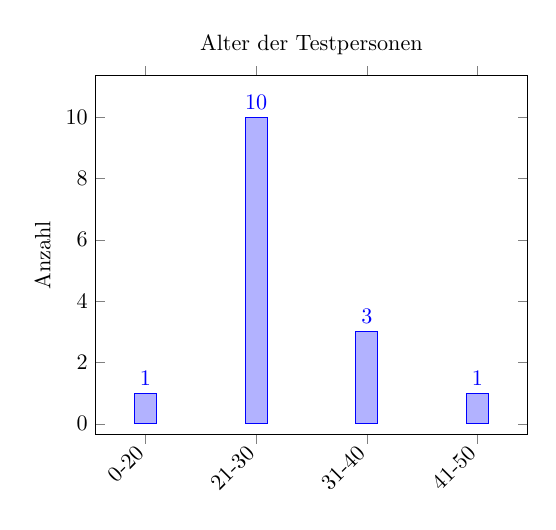
\begin{tikzpicture}[scale=0.8]
  \begin{axis}[
    title=Alter der Testpersonen,
    ybar,
    enlargelimits=0.15,
    legend style={at={(0.5,-0.2)},
      anchor=north,legend columns=-1},
    ylabel={Anzahl},
    symbolic x coords={0-20, 21-30, 31-40, 41-50},
    xtick=data,
    nodes near coords,
	nodes near coords align={vertical},
    x tick label style={rotate=45,anchor=east}]
    \addplot coordinates {(0-20,1) (21-30,10) (31-40,3) (41-50,1)};
  \end{axis}
\end{tikzpicture}
\end{minipage}\qquad
\begin{minipage}[b][6cm][s]{.45\textwidth}
\centering
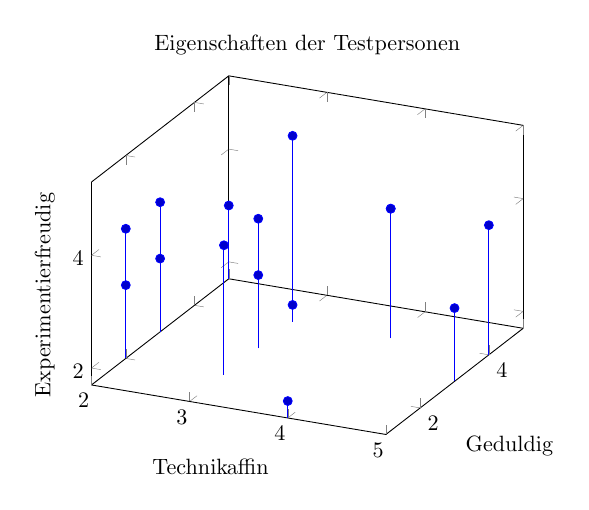
\begin{tikzpicture}[scale=0.8]
\begin{axis}[title=Eigenschaften der Testpersonen,
	xlabel=Technikaffin,
	ylabel=Geduldig,
    zlabel=Experimentierfreudig]
\addplot3+[ycomb]
coordinates
{(2,3,3) (2,5,3) (2,2,4) (2,2,3) (2,3,4) (3,3,3) (3,4,2) (3,4,5) (3,3,4) (3,2,4) (4,4,4)
 (4,1,2) (4,4,4) (5,4,4) (5,3,3)};
\end{axis}
\end{tikzpicture}
\end{minipage}
\end{figure}
\\
Grundsätzlich wurden alle Aufgaben gut gelöst. Die Testpersonen hatten bis auf die Aufgabe mit dem höchsten Komplexitätsgrad keine grösseren Schwierigkeiten. Die Resultate der Fragebogen sind in Abbildung \ref{fig:testresult1} dargestellt.\\[2ex]
%
\begin{figure}[ht]
\caption[Testresultate]{Testresultate}
\label{fig:testresult1}
% Aufgabe 1
%
\begin{minipage}[b][7cm][s]{.45\textwidth}
\centering
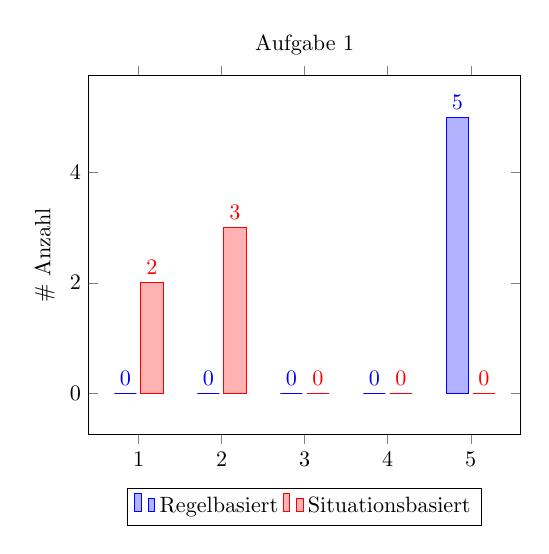
\begin{tikzpicture}[scale=0.8]
\begin{axis}[
    title = Aufgabe 1,
    ybar,
    enlargelimits=0.15,
    legend style={at={(0.5,-0.15)},
    anchor=north,
    legend columns=-1},
    ylabel={\# Anzahl},
    symbolic x coords={1,2,3,4,5},
    xtick=data,
    nodes near coords,
    nodes near coords align={vertical},
    ]
\addplot coordinates {(1, 0) (2,0) (3, 0) (4,0) (5,5)};
\addplot coordinates {(1, 2) (2,3) (3, 0) (4,0) (5,0)};
\legend{Regelbasiert, Situationsbasiert}
\end{axis}
\end{tikzpicture}
\end{minipage}
\qquad
%
% Aufgabe 2
\begin{minipage}[b][7cm][s]{.45\textwidth}
\centering
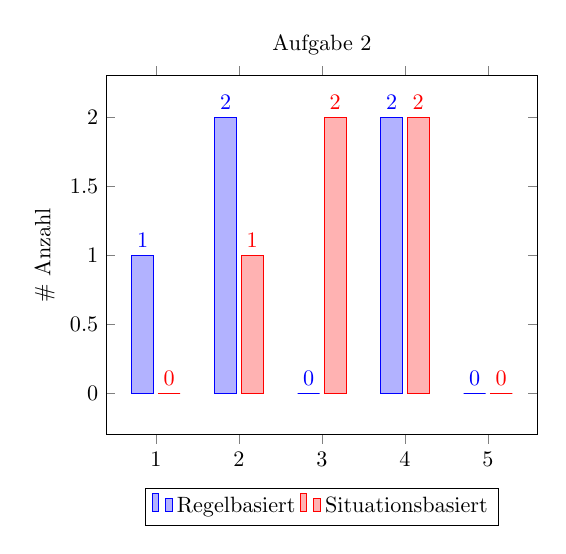
\begin{tikzpicture}[scale=0.8]
\begin{axis}[
    title=Aufgabe 2,
    ybar,
    enlargelimits=0.15,
    legend style={at={(0.5,-0.15)},
      anchor=north,legend columns=-1},
    ylabel={\# Anzahl },
    symbolic x coords={1, 2, 3, 4, 5},
    xtick=data,
    nodes near coords,
    nodes near coords align={vertical},
    ]
\addplot coordinates {(1, 1) (2,2) (3, 0) (4, 2) (5, 0)};
\addplot coordinates {(1, 0) (2,1) (3,2)(4, 2) (5, 0)};
\legend{Regelbasiert, Situationsbasiert}
\end{axis}
\end{tikzpicture}
\end{minipage}
%
% Aufgabe3
\begin{minipage}[b][7cm][s]{.45\textwidth}
\centering
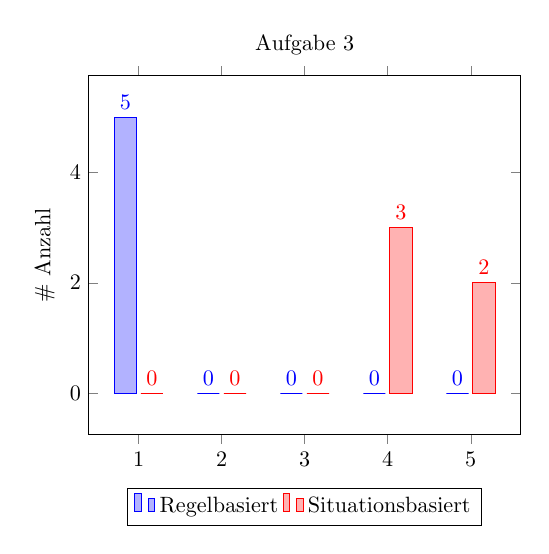
\begin{tikzpicture}[scale=0.8]
\begin{axis}[
    title=Aufgabe 3,
    ybar,
    enlargelimits=0.15,
    legend style={at={(0.5,-0.15)},
      anchor=north,legend columns=-1},
    ylabel={\# Anzahl },
    symbolic x coords={1, 2, 3, 4, 5},
    xtick=data,
    nodes near coords,
    nodes near coords align={vertical},
    ]
\addplot coordinates {(1, 5) (2,0) (3, 0) (4, 0) (5, 0)};
\addplot coordinates {(1, 0) (2,0) (3,0 )(4, 3) (5, 2)};
\legend{Regelbasiert, Situationsbasiert}
\end{axis}
\end{tikzpicture}
%
\end{minipage}
\qquad
%
% Alle Zusammen
% Aufgabe3
\begin{minipage}[b][7cm][s]{.45\textwidth}
\centering
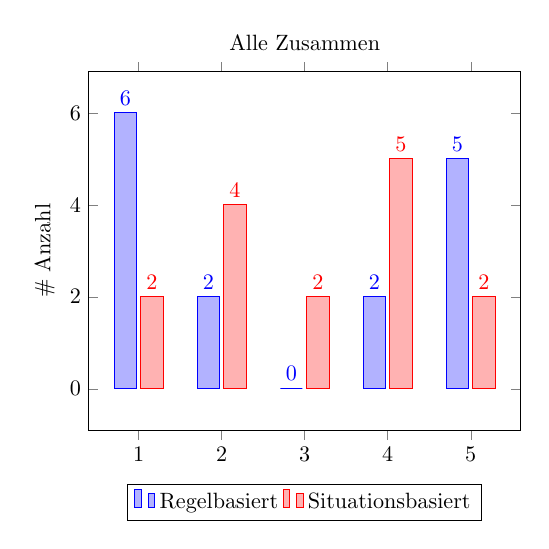
\begin{tikzpicture}[scale=0.8]
\begin{axis}[
    title=Alle Zusammen,
    ybar,
    enlargelimits=0.15,
    legend style={at={(0.5,-0.15)},
      anchor=north,legend columns=-1},
    ylabel={\# Anzahl },
    symbolic x coords={1, 2, 3, 4, 5},
    xtick=data,
    nodes near coords,
    nodes near coords align={vertical},
    ]
\addplot coordinates {(1, 6) (2,2) (3, 0) (4, 2) (5, 5)};
\addplot coordinates {(1, 2) (2,4) (3, 2)(4, 5) (5, 2)};
\legend{Regelbasiert, Situationsbasiert}
\end{axis}
\end{tikzpicture}
%
\end{minipage}
\end{figure}
%
%
Bei der Aufgabe 1 befand die Mehrheit der Testpersonen den regelbasierten Ansatz für geeigneter. Da beim situationsbasierten Ansatz die Testpersonen den Aufwand höher empfanden als beim regelbasierten Ansatz. Zum Teil wurde bemängelt, dass man eine Situation mehrmals bearbeiten musste um die Übergänge zu definieren.\\
Alle Testpersonen konnten sich beide Ansätze ohne Probleme im Kopf vorstellen und die Aufgabe direkt in unserer Webapplikation umsetzen. Somit waren auch alle Testpersonen mit ihrem Ergebnis zufrieden.\\[2ex]
%
Bei der zweiten Aufgabe waren die Meinungen der Testpersonen unterschiedlich. Gewisse Testpersonen fanden den regelbasierten Ansatz besser, da sie sich diese Lösung besser vorstellen konnten. Andere Testpersonen wiederum bevorzugten den situationsbasierten Ansatz, da sie bei diesem eine Trennung zwischen Situationen und Regeln hatten.
Es gab auch Testpersonen, die sich nicht wirklich für einen Ansatz entscheiden konnten und beide Ansätze als gut erachteten.\\
Bei dieser Aufgabe hatten sich gewisse Testpersonen zuerst einen Plan auf Papier gemacht und dann versuchten diesen umzusetzen, während die anderen nach dem \glqq Trial and Error\grqq Prinzip vorgingen. Beide Gruppen konnten die Aufgabe lösen und waren zufrieden mit ihrem Ergebnis.\\[2ex]
%
Die dritte Aufgabe war nicht so leicht zu lösen für die Testpersonen. Zwei Testpersonen sahen sofort, dass der regelbasierte Ansatz nicht funktionieren wird. Die restlichen drei Testpersonen versuchten die Anforderungen umzusetzen, fanden aber keine brauchbaren Lösungen. Beim situationsbasiertem Ansatz konnten nicht alle Testpersonen alle Anforderungen ohne Hilfe umsetzen. Deshalb waren auch nicht alle Testpersonen zufrieden mit ihrem Ergebnis.\\
Bis auf eine Testperson hatten sich alle Notizen gemacht. Zum Teil benötigten die Testpersonen die Notizen um die einzelnen Regeln aufzuschreiben, damit sie nicht immer den ganzen Text lesen müssen.\\
Gewisse Testpersonen stellten zuerst die Situation im Raum her und übernahmen diese dann, mit Hilfe der aktuell angezeigten Sensorwerten, in die Webapplikation.\\[2ex]
%
Allgemein haben die Testpersonen die Webapplikation als verwendbar betrachtet. Einige Benutzer hätten es als hilfreich empfunden, wenn ein Hilfstext angezeigt worden wäre. Andere Testpersonen vermissten eine Zeitdimension. Also eine Angabe ob die Situation für eine gewisse Zeit aktiv ist oder eine Regel wird nur ausgeführt wenn die Zeit stimmt.\\
Was den Testpersonen besonders gut gefiel, war das sofortige Feedback, wenn sich ein Zustand eines Sensor geändert hatte. Das hatte einigen Testpersonen geholfen die einzelnen Regeln zu überprüfen.\\
Ein grosser Teil der Testpersonen fanden das Einrichten nicht mühsam sondern eher unterhaltsam und interessant.
%
% Auswertung nimmt diese Resultate entgegen und gibt antworten auf unsere Fragen.
% Beantworten der Forschungsfrage
% Wie müssen die Resultate gelesen werden
% T- testresult1
% wo ist es statistisch signifikant
% qualitativ argumentieren Aussagen von nutzer nehemn
\subsection{Auswertung}
Es hat sich gezeigt, dass der situationsbasierte Ansatz bei Systemen mit hoher Komplexität besser ist, als der regelbasierte Ansatz. Letzterer wiederum ist besser geeignet bei kleinen, einfachen Systemen.\\
Bei einem einfachen System hatten die Testpersonen den situationsbasierten Ansatz für ungeeignet betrachtet, obwohl sie die Aufgabe richtig lösen konnten. Somit muss die Applikation so einfach wie möglich für den Benutzer verwendbar sein \cite{ifttt}. Kann er eine Situation nicht fertig einrichten, da ihm die Übergänge fehlen, kommt ihm das als mühsam, beziehungsweise kompliziert, vor. Das Festlegen von unkomplizierten Regeln soll somit rasch und einfach möglich sein.\\
Die ausgewerteten Daten mit einem T-Test für die Aufgabe 1 werden in Tabelle \ref{tab:auf1} gezeigt. Diese zeigen deutlich, dass der regelbasierte Ansatz bevorzugt wird gegenüber dem situationsbasierten Ansatz.  Die Resultate haben eine statistische Signifikanz von 0.0010.\\[2ex]
\begin{table}[h]
\centering
\begin{tabular}{@{} l | c | c @{}}
 & regelbasierter Ansatz & situationsbasierter Ansatz \\ \hline
 Mean & 4.8  & 1.6  \\ \hline
 SD & 0.45  & 0.55  \\ \hline
 SEM & 0.2  & 0.24  \\ \midrule
 \end{tabular}
\caption{\label{tab:auf1}T-Test Aufgabe 1}
\end{table}
% Platform muss ihn unterstützen und nicht hindern

Werden die Systeme komplexer, können aber noch mit dem regelbasierten Ansatz gelöst werden, gibt es keinen eindeutig geeigneten Ansatz. Das zeigt auch die statistische Signifikanz bei der Auswertung. Diese liegt bei 0.53. Auch fiel es den Testbenutzern schwer sich für einen Ansatz zu entscheiden. So hatte ein User geschrieben: \enquote{(...)Ich finde es noch schwer zu sagen, was mir besser gefällt.(...)}. Es ist somit davon auszugehen, dass es auf die persönliche Präferenz des Benutzers und die zur Verfügung stehende Plattform ankommt, welchen Ansatz er für besser geeignet hält\cite{gut}. Tabelle \ref{tab:auf2} zeigt die Auswertung des T-Tests für die zweite Aufgabe.\\[2ex]
\begin{table}[h]
\centering
\begin{tabular}{@{} l | c | c @{}}
 & regelbasierter Ansatz & situationsbasierter Ansatz  \\ \hline
 Mean & 2.6  & 3.2  \\ \hline
 SD & 1.34  & 0.84  \\ \hline
 SEM & 0.6  & 0.37  \\ \midrule
 \end{tabular}
\caption{\label{tab:auf2}T-Test Aufgabe 2}
\end{table}

Handelt es sich um ein System mit hoher Komplexität fällt der regelbasierte Ansatz durch. Oder wie es eine Testperson beschrieb: \enquote{Ansatz 1 (A.d.V: regelbasierte Ansatz) war nicht möglich umzusetzen.}. Hier zeigen sich die Stärken des situationsbasierten Ansatz. Die Applikation abstrahiert das System und hilft dem Benutzer eine Übersicht zu behalten. Eine Applikation sollte deswegen, wo immer möglich, die Komplexität verringern und somit den Benutzer bei seiner Umsetzung unterstützen\cite{simple, gut2} .\\
Das Nachstellen oder Aufzeichnen von Situationen zeigt, dass eine Applikation die verschiedenen Umsetzungsstrategien der Benutzer anbieten sollte. Dies ist bei einem situationsbasierten Ansatz gut möglich, da man Situationen und Regeln trennen kann.\\
Tabelle \ref{tab:auf3} zeigt die Resultate der Aufgabe 3. Die statistische Signifikanz liegt bei 0.0002.\\[2ex]
\begin{table}[h]
\centering
\begin{tabular}{@{} l | c | c @{}}
 & regelbasierter Ansatz & situationsbasierter Ansatz \\ \hline
 Mean & 1  & 4.4  \\ \hline
 SD & 0  & 0.55  \\ \hline
 SEM & 0  & 0.24  \\ \midrule
 \end{tabular}
\caption{\label{tab:auf3}T-Test Aufgabe 3}
\end{table}
% Übersichtlich = regelbasiert
% einfache IFTTT
% Komplex Verknüpft oder sensoren mehrmals verwendet = situationsbasiert.
% Feedback ist wichtig für den User Trial and errro
% Zum Teil schwierigkeiten mit Übergängen.
% Wieso wir nur die letzten Angeschaut
% Wieso haben nur die Personen diese preferenzen => Kommentare eingehen

Allgemein sollte die Applikation transparent sein. Damit der Benutzer zu jeder Zeit weiss, wie sich das System verhält. Es hat sich gezeigt, dass ein direktes Feedback der Sensoren für den Benutzer sehr angenehm ist. Der Benutzer kann so sein System nach und nach aufbauen und direkt überprüfen. Auch das Anzeigen des aktuellen Status eines Sensors hilft dem Benutzer sein System besser zu verwalten. Allgemein möchte der User eine gute Übersicht über sein System haben.\cite{gut2, gut}
%
%
% Nur 5 Probanden Keine statistischen Test die aussagbar sind
% Nicht normalverteilt
% Test ist nicht zuverlässig
% Algemein gültig sind die Probanden representativ ist das Szenario representativ
% Interne validierung haben wir probanden beeinflusst
% - > was haben wir glaubwürdig gemacht
% Hat es Personen gestunken
\subsection{Gültigkeitsrisiken}
In dieser Studie gilt es natürlich zu beachten, dass insgesamt nur 15 Teilnehmer dabei waren. Somit wurde eine Aufgabe von fünf Testpersonen durchgeführt. Die Testergebnisse haben daher nur eine bedingte statistische Aussage. Des Weiteren ist es möglich, dass die Testpersonen von uns beeinflusst wurden, als wir ihnen die beiden Ansätze vorgestellt hatten. So könnte es sein, dass sie den Fragebogen zu unseren Gunsten ausgefüllt hatten. Wir hatten uns jedoch stets bemüht neutral zu bleiben und keinen Ansatz in einem positiven oder einem negativen Licht darzustellen.\\
Da alle Testpersonen Spass bei der Durchführung hatten, gehen wir nicht davon aus, dass Testpersonen mit Absicht falsche Antworten gaben um das Resultat zu verfälschen. Die Testpersonen sehen wir als repräsentativ, da sie kein spezifisches Fachwissen oder Expertise im Bereich IoT mit brachten.\\
Die Aufgaben sind erfunden und stammen nicht von einem realen Beispiel. Es gibt aber sicher ähnliche Systeme und somit sind die Aufgaben realistisch.